%!TEX root = ../main.tex
\section{NGT--DAQ Integration} % Thiago

%%% We just write the discussion we had in the whole DAQ session

The Optimal Calibration system has to be embedded in the CMS trigger and data acquisition (DAQ) system,
both in the demonstrator system and in the \Phasetwo implementation.
We briefly review the DAQ system architecture implemented for \Runthree, 
compare it tow the baseline DAQ architecture proposed for \Phasetwo, and 
go through a preliminary calculation of the NGT system feasibility.
We finally discuss a minimal implementation of the demonstrator and
how it can be integrated in the \Runthree system.

\subsection{Demonstrator Integration in Run 3}

The CMS DAQ system for Run 3 (DAQ3) is an intricate system, dealing with all steps of the data flow from the sub-detector front-end drivers (FEDs) through the final delivery of data streams to Tier-0. For the purposes of our discussions, we can focus on the following elements of Figure~\ref{fig:DAQ3}: 
the \emph{Readout Units} (RUs) unpack and merge event fragments into super-fragments, which are then sent to the \emph{Builder Units} (BUs) to be further assembled into complete events. 
The complete events are sent to the \emph{Filter Units} (FUs), where the HLT application runs and selects a subset of the events to be saved for permanent storage. 
In the DAQ3 implementation, the RUs and the BUs are logically separate, but physically realised in the same computer node.
\begin{figure}[htbp]
   \centering
	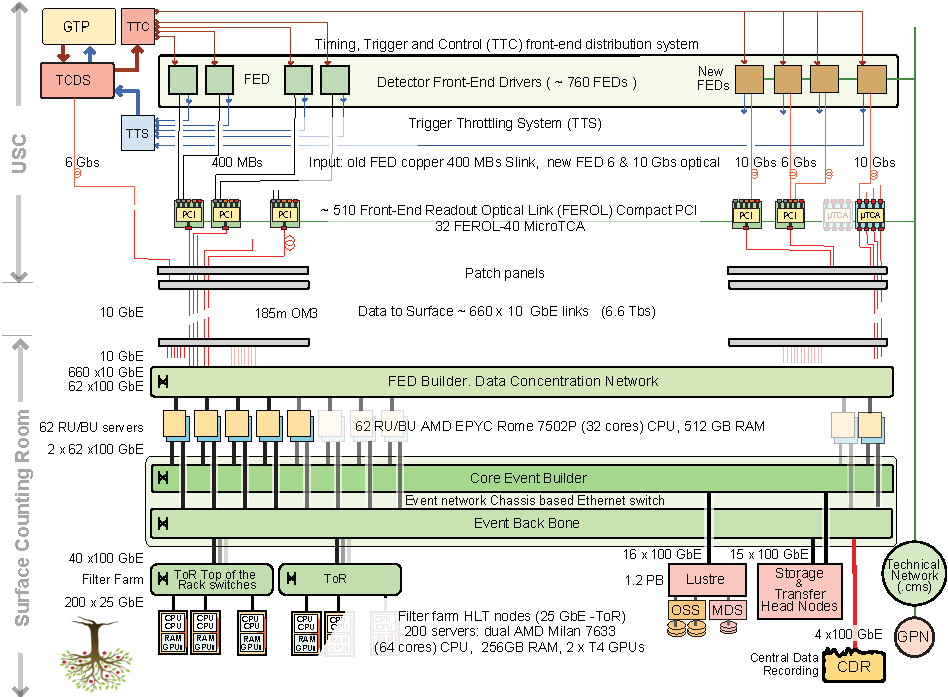
\includegraphics[width=0.7\textwidth]{figures/DAQRun3.pdf}
  \caption{Diagram of the \Runthree DAQ system.}
   \label{fig:DAQ3}
\end{figure}

The output data are then sent back to the BUs, where they are further merged and their management is handed over to the storage and transfer system (STS).
The STS  transfers the data to a (Lustre-based) cluster file system, whence they are finally sent to their final destination:
Tier-0,
DQM
or the calibration cluster.
The DAQ3 was also designed with two characteristics that the demonstrator should respect: 
i) it is \emph{pipelined}, so the data should follow an unidirectional flow;
ii) it is \emph{democratic}, in the sense that all elements (RUs, BUs, FUs) are treated equally.

%%% Thiago testing the GitHub integration
% I want to work at the LHC!
% I want to work at the FCC!

\subsection{Baseline DAQ Architecture for \Phasetwo}

The baseline architecture for  the \Phasetwo DAQ system is shown in Figure~\ref{fig:DAQP2}.
A comparison with Fig.~\ref{fig:DAQ3} shows that it is a direct evolution of the \Runtwo system,
upgraded to be withstand the larger data flows of the HL-LHC era.
This makes the necessity of a demonstrator system even more pressing.

\begin{figure}[htbp]
   \centering
	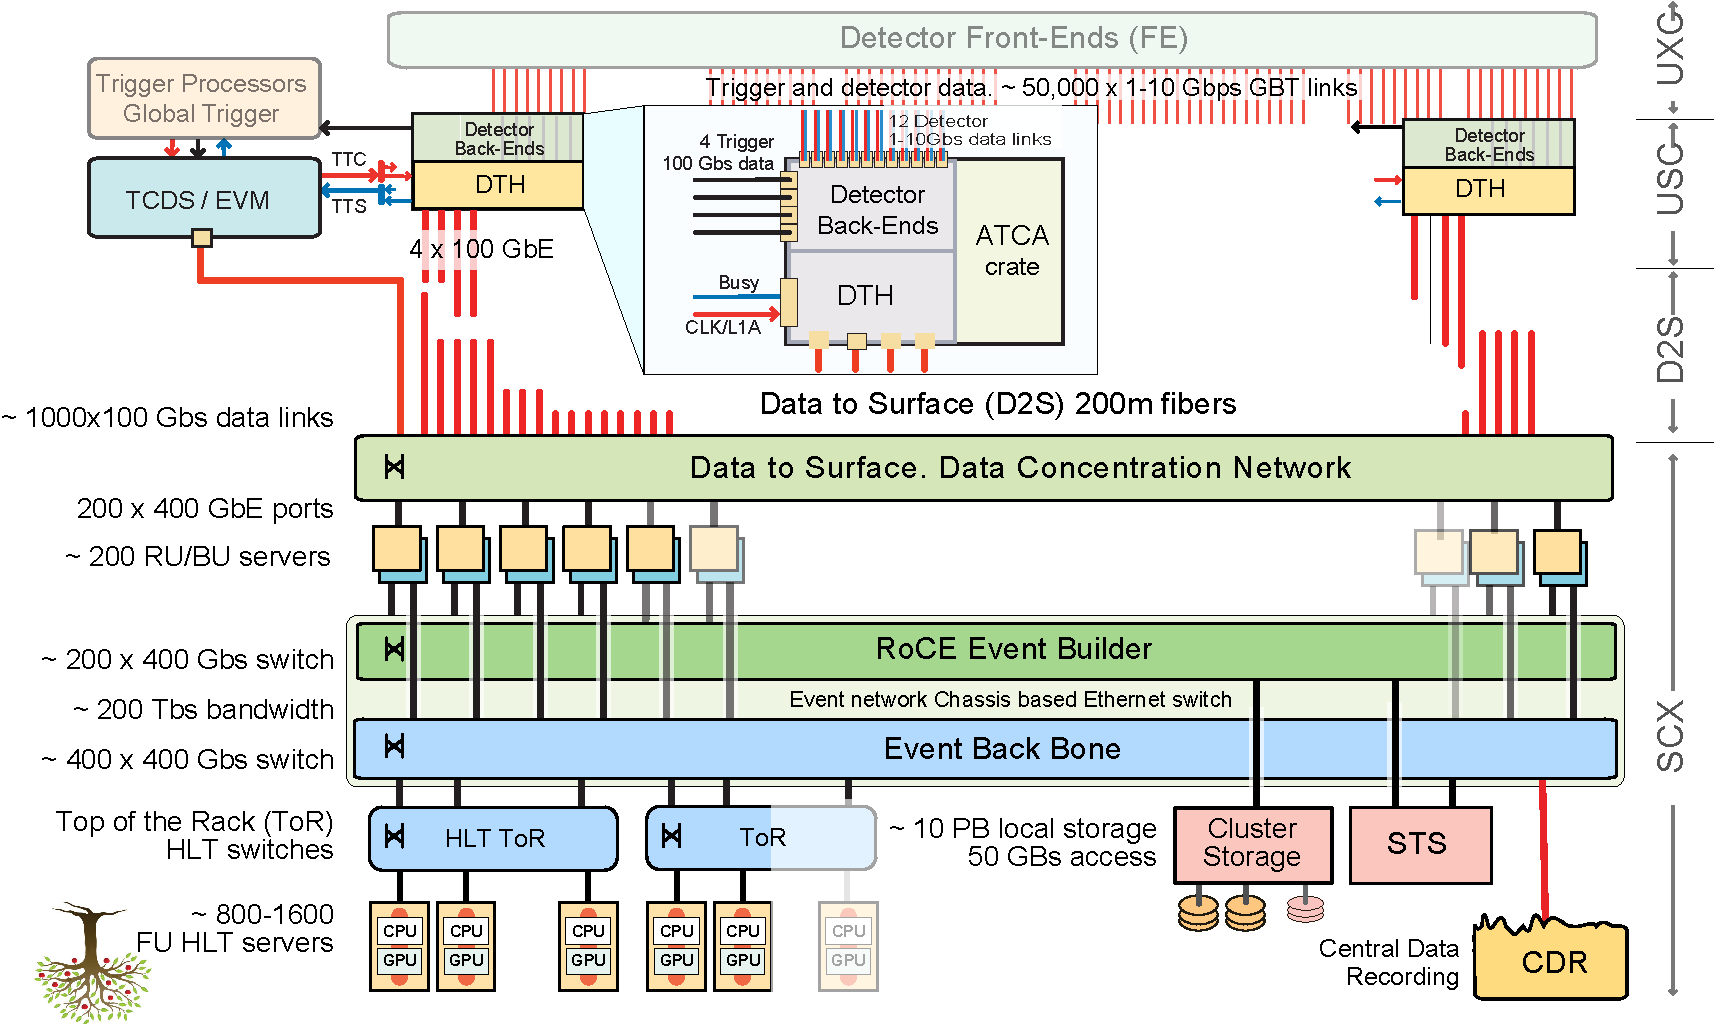
\includegraphics[width=0.7\textwidth]{figures/Phase2-Layout-1-20210913.pdf}
}
  \caption{Conceptual diagram of the \Phasetwo DAQ system.}
   \label{fig:DAQP2}
\end{figure}


\subsection{System Feasibility: Preliminary Calculation}

As the overarching goal of the NGT project is to reconstruct and save all the L1-accepted data, 
our first assumption is that 
\emph{the system will have to buffer all the data of a run whilst running the optimal calibrations}.
The size of the data buffer $B$ can be estimated by the following formula
\begin{equation}
B = R \times \tau \times E \times s
\label{eq:buffersize}
\end{equation}
where $R$ is the input rate to the buffer,
$\tau$ is the period during which we have to buffer the data,
$E$ is the event size and
$s$ is a safety factor.
For a first calculation, we take the Run 4 estimates from the DAQ-HLT TDR:
$R = A^\text{L1}$ = 500\kHz, $E$ = 6.1\MB,
and assume a flat 50\% safety factor ($s$ = 1.5).
The discussion on the magnitude of the buffer period $\tau$ is more subtle and will be done in the next section.

\subsubsection{Buffer Period}

The amount of time during which the data has to be buffered depends on many factors,
and we add a set of working hypotheses to be able to estimate its value.
\begin{itemize}
\item The buffer period has to be longer than the amount of time needed to derive the calibrations.
A relevant timescale is the PCL completion time, which we know from experience to take close to eight hours.
We know from experience that the PCL takes, in average, 8 hours to run for completion.
Some of the longest runs, however, may need additional time; a long run from LHC fill 10200 took data during more than 13 hours
(delivering close to $900\pbinv$), and
the PCL took more than 10 hours to finish,
as seen in Fig.~\ref{fig:fill10200PCL}.
Notice that, in offline reconstruction, Tier-0 starts the PCL only after the run end; 
therefore the 48 hours limit for the start of prompt reconstruction applies to 
the sum of run duration and the PCL duration.
After the calibration is done the data has to be buffered for some more time in order to allow the NGT reconstruction to run.
Therefore, we choose to use a representative value of \emph{12 hours}.
\begin{figure}[htbp]
   \centering
	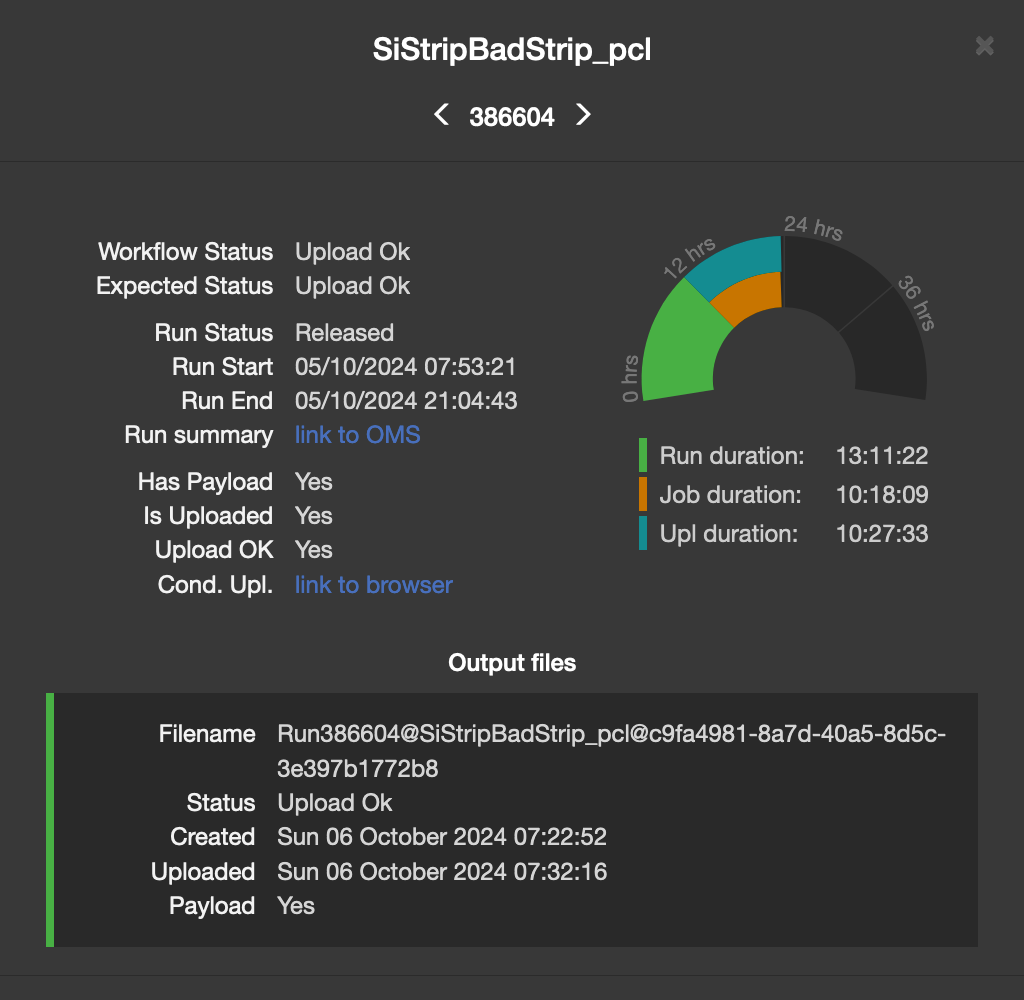
\includegraphics[width=0.7\textwidth]{figures/fill10200PCL.png}
   \caption{PCL monitoring of the silicon strip bad components calibration for a run of LHC fill 10200 (the number 386604 refers to internal CMS bookkeeping).
   The run took data over more than 13 hours, whilst the PCL ran for over 10 hours.}
   \label{fig:fill10200PCL}
\end{figure}
\item On the other hand, the buffer has to be large enough to store all the data from an LHC fill, as per our first assumption,
but that calculation has to take into account the LHC duty cycle, so we use the following working hypotheses:
\begin{itemize}
\item The High-Luminosity LHC will work in a $\sim70\%$ duty cycle, meaning that in a 24-hour period there will be 17 hours of stable beams and 7 hours of interfill (including injection and ramp).
\item Levelling will once again be used to keep the effective luminosity at a given level.
Following the Run 3 historic performance, we assume that the 17 hours of stable beams will be divided into 10 hours of levelling and 7 hours of lumi decay phase.
\item Again following the Run 3 performance, we assume that the luminosity (as well as the pileup) in the decay phase will average out to $\sim80\%$ of levelled luminosity.
\item We assume that the event size $E$ scales linearly with pileup.
\item We assume that the Level-1 accept rate $A^{\text{L1}}$ will be kept constant even during the decay phase. 
\item The 7 hours of downtime are effectively free from the point of view of data buffering for NGT.
\end{itemize}
\end{itemize}

By simply substituting $\tau$ = 12 hours in Eq.~\ref{eq:buffersize}, we arrive at a buffer size $B = 200\PB$.
The second calculation that accounts for the LHC duty cycle amounts to three applications of the same equation,
and is summarised in Table~\ref{tab:bufferWithDutyCycle}. In that case, we arrive at a buffer size of $B = 258\PB$ for a 24 hour period.
Noting that the two results agree within $\sim25\%$, and that many more assumptions go into the second calculation, for the purposes of this report we proceed with the \textbf{200\,PB} figure.
% Requires the booktabs if the memoir class is not being used
\begin{table}[htbp]
   \centering
   %\topcaption{Table captions are better up top} % requires the topcapt package
   \begin{tabular}{@{} lrrrrr @{}} % Column formatting, @{} suppresses leading/trailing space
      \toprule
		Phase & Duration (h) & $A^{\text{L1}}$ (\kHz) & $E$ (\MB) & Safety factor & Buffer (\PB)\\
      	\midrule
		Levelling & 10 & 500 & 6.1 & 1.5 & 165 \\
		Decay     &  7 & 500 & 4.9 & 1.5 &  93 \\
		Interfill &  7 &  -- &  -- &  -- &   0 \\
		\midrule
\textbf{Total}    & 24 & N/A & N/A & N/A & 258\\ 
      \bottomrule
   \end{tabular}
   \caption{Calculation for NGT buffer size accounting for LHC duty cycle. 
   This modelling concludes that a 258\,PB buffer is adequate for a 24-hour period.}
   \label{tab:bufferWithDutyCycle}
\end{table}

We can compare the proposed NGT buffer size to a number of similar systems.
The current storage capacity of the CMS Run 3 DAQ system is 1.2\,PB.
The LHCb experiment implemented a similar dataflow in their DAQ system, 
with events accepted by their HLT1 system held in a 30\,PB buffer,
used for real-time alignment and calibration,
and finally passed on to their HLT2 system.
\textcolor{red}{The the CMS Tier-0 holds a disk buffer of 11\,PB for incoming raw data from Point 5 to be held on for prompt reconstruction,
as well as a disk buffer of $25\PB$ for reconstructed data before it is transferred to other sites in the WLCG.}
We also note that experience from the LHCb system shows that the reading/writing speed of the disks decreases when they fill up,
which justifies the consideration of a large safety factor ($s = 1.5$).

Finally, we note that the physical location of the buffer is yet to be defined.
There are three possibilities: 
locally attached to a BU, to a FU, or as a separated central storage.
For a preliminary estimation, we assume the ``buffer attached to FU'' scenario.
According to the DAQ-HLT TDR,
1600 (840) rack-mount 1U (2U) servers would comprise the HLT farm for \Runfour (\Runfive).
If it were feasible to use the latter configuration for \Runfour as well,
the problem would be how to divide 200 PB in 840 2U servers.
That comes down to  $240\TB$ per server; $60\TB$ disks have recently become available today~\cite{micron60tb},
and there is a high probability that $120\TB$ disks will be available for \Runfour.
So this scenario can be realised by installing two extra disks in each server of the HLT farm.

\subsubsection{Nodes for the Optimal Calibration}

The computer nodes for the optimal calibration (henceforth ``calibration nodes'') have to be integrated in the DAQ system.
The alignment and calibration algorithms need built events to run over, so these nodes need to be downstream of the BUs.
It is easiest to locate these nodes downstream of the FUs as well --
in this way, the FUs can naturally transmit the necessary data streams to the calibration nodes, 
just as they do for the offline calibrations.

\subsubsection{Additional Output to the Storage and Transfer System}

The additional bandwidth needed to sustain the output data stream of the NGT workflow also imposes requirements on the Phase-2 DAQ system.
Assuming we will save all the L1T-accepted events in a reduced data format comparable to the current Scouting format~\cite{CMS:2024zhe},
%%% Thiago: should we somehow talk about Task 3.3 here?
this will lead to an additional output of $500\kHz 
\times 25\,\text{kB}$ = $12.5\GBpers$.
This is comparable in magnitude, albeit smaller, to the 51\,GB/s quoted for the storage throughput in the DAQ-HLT TDR.

\subsection{Minimum Minimorum NGT Demonstrator}

In view of the discussion above, a minimal NGT demonstrator would take the following form:
\begin{itemize}
\item \textbf{The standard HLT runs as normal.} 
The capability to run without interfering with the regular data-taking is
a non-negotiable characteristic of the demonstrator.
\item \textbf{A prescaled copy of the Scouting input data stream is added to the HLT menu.}
The input to the Scouting is solely defined by the logical OR of a set of L1T seeds, and
selecting events based on that requirement is a very cheap operation in terms of computing resources.
A reasonable prescale could be $\mathcal{O}(100)$, reducing the data stream 
from $\sim 30\kHz$
to $\sim 300\kHz$.
\item \textbf{We buffer the resulting data set for 48 hours.}
For the demonstrator we take the absolute worst case scenario of the alignment and calibration algorithms taking the same time to run as those in the PCL.
In terms of the Run 3 DAQ system, this machine would simply be configured as another stream destination.
\item \textbf{A copy of the data streams needed for the candidate calibrations is added to the HLT menu.}
For the candidate calibrations, we estimate that 
%%% Thiago: to be cross-checked
the data from ``Express'', ``ExpressAlignment'' and ``Calibration'' streams should suffice.
Those streams amount to an additional rate of $\sim 300\Hz$.
Together with the previous point, we
use Eq.~\ref{eq:buffersize}, using 
$R = 600\Hz$,
$\tau$ = 48 h,
$E = 1.2\MB$ and
$s$ = 1.5
would entail a buffer of $\sim 200\TB$.
A regular HLT-class node with four $60\TB$ disks should be able to hold the data easily.
\item \textbf{We use the regular workflows to derive the candidate calibrations.}
Another machine, similar to the first, accesses the demonstrator data buffer
and
runs the alignment and calibration algorithms.
\item \textbf{Re-run the Scouting paths on the buffered data with the updated calibrations.}
The framework for rerunning the HLT with an alternate set of calibration has already been discussed in Section~\ref{sec:}.
\item \textbf{Compare the performance of the original vs re-run Scouting.}
This should demonstrate the effect of the updated calibrations. 
\end{itemize}


